\tikzset{every picture/.style={line width=0.75pt}} %set default line width to 0.75pt        

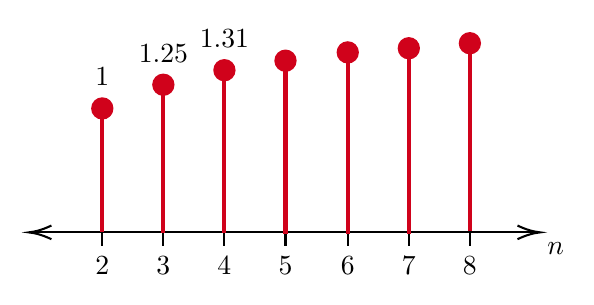
\begin{tikzpicture}[x=0.75pt,y=0.75pt,yscale=-1,xscale=1]
%uncomment if require: \path (0,412); %set diagram left start at 0, and has height of 412

%Straight Lines [id:da8584009914648288] 
\draw    (419.71,195) -- (177.29,195) ;
\draw [shift={(175.29,195)}, rotate = 360] [color={rgb, 255:red, 0; green, 0; blue, 0 }  ][line width=0.75]    (10.93,-3.29) .. controls (6.95,-1.4) and (3.31,-0.3) .. (0,0) .. controls (3.31,0.3) and (6.95,1.4) .. (10.93,3.29)   ;
\draw [shift={(421.71,195)}, rotate = 180] [color={rgb, 255:red, 0; green, 0; blue, 0 }  ][line width=0.75]    (10.93,-3.29) .. controls (6.95,-1.4) and (3.31,-0.3) .. (0,0) .. controls (3.31,0.3) and (6.95,1.4) .. (10.93,3.29)   ;
%Straight Lines [id:da9886964674804183] 
\draw    (299,189.29) -- (299,201.71) ;
%Straight Lines [id:da8156036240841317] 
\draw    (329,189.29) -- (329,201.71) ;
%Straight Lines [id:da7338901612135262] 
\draw    (358.42,189.29) -- (358.42,201.71) ;
%Straight Lines [id:da44762648985303743] 
\draw    (387.84,189.29) -- (387.84,201.71) ;
%Straight Lines [id:da9635121855917483] 
\draw    (269.58,189.29) -- (269.58,201.71) ;
%Straight Lines [id:da9816533416924345] 
\draw    (240.16,189.29) -- (240.16,201.71) ;
%Straight Lines [id:da026365304419259328] 
\draw    (210.74,189.29) -- (210.74,201.71) ;
%Straight Lines [id:da36890566565614835] 
\draw [color={rgb, 255:red, 208; green, 2; blue, 27 }  ,draw opacity=1 ][line width=1.5]    (210.74,135.29) -- (210.74,194.71) ;
\draw [shift={(210.74,135.29)}, rotate = 90] [color={rgb, 255:red, 208; green, 2; blue, 27 }  ,draw opacity=1 ][fill={rgb, 255:red, 208; green, 2; blue, 27 }  ,fill opacity=1 ][line width=1.5]      (0, 0) circle [x radius= 4.36, y radius= 4.36]   ;
%Straight Lines [id:da7429942794858413] 
\draw [color={rgb, 255:red, 208; green, 2; blue, 27 }  ,draw opacity=1 ][line width=1.5]    (240.16,123.87) -- (240.16,195.29) ;
\draw [shift={(240.16,123.87)}, rotate = 90] [color={rgb, 255:red, 208; green, 2; blue, 27 }  ,draw opacity=1 ][fill={rgb, 255:red, 208; green, 2; blue, 27 }  ,fill opacity=1 ][line width=1.5]      (0, 0) circle [x radius= 4.36, y radius= 4.36]   ;
%Straight Lines [id:da27787186266965624] 
\draw [color={rgb, 255:red, 208; green, 2; blue, 27 }  ,draw opacity=1 ][line width=1.5]    (269.58,116.87) -- (269.58,195.29) ;
\draw [shift={(269.58,116.87)}, rotate = 90] [color={rgb, 255:red, 208; green, 2; blue, 27 }  ,draw opacity=1 ][fill={rgb, 255:red, 208; green, 2; blue, 27 }  ,fill opacity=1 ][line width=1.5]      (0, 0) circle [x radius= 4.36, y radius= 4.36]   ;
%Straight Lines [id:da3329910181884447] 
\draw [color={rgb, 255:red, 208; green, 2; blue, 27 }  ,draw opacity=1 ][line width=1.5]    (299,112.29) -- (299,195.71) ;
\draw [shift={(299,112.29)}, rotate = 90] [color={rgb, 255:red, 208; green, 2; blue, 27 }  ,draw opacity=1 ][fill={rgb, 255:red, 208; green, 2; blue, 27 }  ,fill opacity=1 ][line width=1.5]      (0, 0) circle [x radius= 4.36, y radius= 4.36]   ;
%Straight Lines [id:da15731918285032842] 
\draw [color={rgb, 255:red, 208; green, 2; blue, 27 }  ,draw opacity=1 ][line width=1.5]    (329,108.29) -- (329,195.71) ;
\draw [shift={(329,108.29)}, rotate = 90] [color={rgb, 255:red, 208; green, 2; blue, 27 }  ,draw opacity=1 ][fill={rgb, 255:red, 208; green, 2; blue, 27 }  ,fill opacity=1 ][line width=1.5]      (0, 0) circle [x radius= 4.36, y radius= 4.36]   ;
%Straight Lines [id:da49004574560078384] 
\draw [color={rgb, 255:red, 208; green, 2; blue, 27 }  ,draw opacity=1 ][line width=1.5]    (358.42,106.29) -- (358.42,195.71) ;
\draw [shift={(358.42,106.29)}, rotate = 90] [color={rgb, 255:red, 208; green, 2; blue, 27 }  ,draw opacity=1 ][fill={rgb, 255:red, 208; green, 2; blue, 27 }  ,fill opacity=1 ][line width=1.5]      (0, 0) circle [x radius= 4.36, y radius= 4.36]   ;
%Straight Lines [id:da8874563427293995] 
\draw [color={rgb, 255:red, 208; green, 2; blue, 27 }  ,draw opacity=1 ][line width=1.5]    (387.84,103.87) -- (387.84,194.29) ;
\draw [shift={(387.84,103.87)}, rotate = 90] [color={rgb, 255:red, 208; green, 2; blue, 27 }  ,draw opacity=1 ][fill={rgb, 255:red, 208; green, 2; blue, 27 }  ,fill opacity=1 ][line width=1.5]      (0, 0) circle [x radius= 4.36, y radius= 4.36]   ;

% Text Node
\draw (210.74,205.11) node [anchor=north] [inner sep=0.75pt]    {$2$};
% Text Node
\draw (240.16,205.11) node [anchor=north] [inner sep=0.75pt]    {$3$};
% Text Node
\draw (269.58,205.11) node [anchor=north] [inner sep=0.75pt]    {$4$};
% Text Node
\draw (299,205.11) node [anchor=north] [inner sep=0.75pt]    {$5$};
% Text Node
\draw (329,205.11) node [anchor=north] [inner sep=0.75pt]    {$6$};
% Text Node
\draw (358.42,205.11) node [anchor=north] [inner sep=0.75pt]    {$7$};
% Text Node
\draw (387.84,205.11) node [anchor=north] [inner sep=0.75pt]    {$8$};
% Text Node
\draw (423.71,198.4) node [anchor=north west][inner sep=0.75pt]    {$n$};
% Text Node
\draw (210.74,125.89) node [anchor=south] [inner sep=0.75pt]    {$1$};
% Text Node
\draw (240.16,114.47) node [anchor=south] [inner sep=0.75pt]    {$1.25$};
% Text Node
\draw (269.58,107.47) node [anchor=south] [inner sep=0.75pt]    {$1.31$};


\end{tikzpicture}
